\lecture{Sistema de arquivos do Windows}

\begin{frame}{Conceitos básicos}
  \begin{description}
  \item[Setor:] blocos endereçados pelo hardware em um meio de
    armazenamento. Discos rígidos normalmente possuem blocos de 512
    bytes, mas discos com setores de 4.096 bytes estão sendo vendidos.\pause
  \item[Formato:] o formato dos sistemas de arquivos define o modo que 
    os arquivos de dados são armazenados. \pause
  \item[Cluster:] são agrupamentos de setores para aumentar a eficiência 
    do gerenciamento do espaço em disco.\pause
  \item[Metadados:] dão suporte aos sistemas de arquivos no gerenciamento 
    de arquivos e diretórios.
  \end{description}
\end{frame}

\begin{frame}{Formatos de sistemas de arquivos do Windows}
  
  O Windows dá suporte aos seguintes formatos:

  \begin{itemize}
  \item CDFS;
  \item UDF ({\em Universal Disk Format});
  \item FAT12, FAT16 e FAT32;
  \item exFAT (FAT64);
  \item NTFS.
  \end{itemize}
\end{frame}

\begin{frame}{FAT\{12,16,32\}}
  \small
  \begin{itemize}
  \item O sistema FAT existe para manter compatibilidade com sistemas
    multi-boot e dispositivos de armazenamento portáteis.\pause
  \item O número na frente do nome indica o número de bits do endereço
    dos {\em clusters}. Por exemplo, FAT12 indentifica o cluster com
    12 bits, limitando a partição a um máximo de $2^{12}$ (4.096)
    clusters. O Windows permite tamanhos de cluster de 0,5KB a
    8KB.\pause
  \item O volume FAT possui a seguinte organização:
  \end{itemize}

  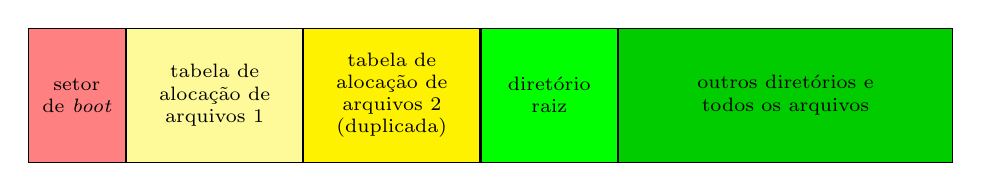
\begin{tikzpicture}[
    every node/.style={minimum height=1.7cm,font=\scriptsize,text centered,draw}
    ]
    
    \node[fill=red!50!white,text width=1cm,draw] (boot) {setor de \em boot};
    \node[fill=yellow!40!white,text width=2cm,right of=boot,xshift=.75cm] (alloc1) {tabela de alocação de arquivos 1};
    \node[fill=yellow,text width=2cm,right of=alloc1,xshift=1.25cm] (alloc2) {tabela de alocação de arquivos 2 (duplicada)};
    \node[fill=green,text width=1.5cm,right of=alloc2,xshift=1cm] (root) {diretório raiz};
    \node[fill=green!80!black,text width=4cm,right of=root,xshift=2cm] {outros diretórios e todos os arquivos};
  \end{tikzpicture}

  \bigskip
  Em caso de corrupção da tabela de alocação de arquivos~1, a tabela~2 é usada.
\end{frame}

\begin{frame}{FAT16}{Tamanho dos {\em clusters}}
  Valores do tamanho padrão para cada cluster, de acordo com o tamanho
  da partição para o FAT16.

  \begin{center}
    \begin{tabular}[ht]{|l|l|}\hline
      \bf tamanho da partição & \bf tamanho padrão do {\em cluster} \\\hline
      <8MB & não suportado\\\hline
      8MB--32MB & 512 bytes\\\hline
      32MB--64MB & 1KB\\\hline
      64MB--128MB & 2KB\\\hline
      128MB--256MB & 4KB\\\hline
      256MB--512MB & 8KB\\\hline
      512MB--1.024MB & 16KB\\\hline
      1GB--2GB & 32KB\\\hline
      2GB--4GB & 64KB\\\hline
      >4GB & não suportado \\\hline
    \end{tabular}
  \end{center}

\end{frame}

%% Fonte: ``Windows Internals 2''', posição 9301

\begin{frame}{NTFS}{Características}
  O NTFS ({\em New Technology File System}) implementa de sistemas de
  arquivos para o SO Windows\textsuperscript{\textregistered}. Algumas
  de suas características são:

  \begin{itemize}
  \item<1> Endereço de cluster de 64 bits.
  \item<2> Segurança de arquivos e diretórios;
  \item<3> Suporte a transação;
  \item<4> Tolerante a falhas através da alteração dos metadados 
    usando transação;
  \item<5> Auto-reparo com o sistema rodando;
  \item<6> Suporte a bloqueio e permissões.
  \end{itemize}  
\end{frame}

\begin{frame}{NTFS}{Tamanho dos {\em clusters}}
  Valores do tamanho padrão para cada cluster, de acordo com o tamanho
  da partição para o NTFS.
  \begin{center}
    \begin{tabular}[ht]{|l|l|}\hline
      \bf tamanho da partição & \bf tamanho padrão do {\em cluster} \\\hline
      <7MB & não suportado\\\hline
      7MB--16TB & 4KB\\\hline
      16TB--32TB & 8KB\\\hline
      32TB--64TB & 16KB\\\hline
      64TB--128TB & 32KB\\\hline
      128TB--256TB & 64KB\\\hline
    \end{tabular}
  \end{center}
\end{frame}

\begin{frame}{Características avançadas do NTFS, parte 1/3}
  \footnotesize
  \begin{description}
  \item<1>[Unicode:]  suporte a caracteres Unicode 1.0/UTF16 de 16~bits para armazenar 
    nomes de arquivos diretórios e volumes.
  \item<2>[Indexação:] Qualquer atributo de arquivo pode ser indexado
    usando a estrutura {\em B-tree}, que permite acesso eficiente ao
    dado. Ao contrário do FAT que indexa mas não ordena os atributos.
    (Não disponível ao usuário)
  \item<3>[{\em Hard link}:] permite que vários caminhos referenciem o
    mesmo arquivo. Por exemplo, se for criado um {\em hard link} de
    {\tt
      C:$\backslash$$\backslash$Documents$\backslash$Relatório.doc}
    para {\tt
      C:$\backslash$$\backslash$Users$\backslash$Administrador$\backslash$Documents$\backslash$Relatório.doc},
    os dois links referem-se ao mesmo arquivo no disco.
  \end{description}
\end{frame}

\begin{frame}{Características avançadas do NTFS, parte 2/3}
  \footnotesize
  \begin{description}
  \item<1>[{\em Link} simbólico:] {\em strings} que são interpretadas
    dinamicamente e podem ser caminhos relativo ou absoluto em
    qualquer dispositivo de armazenamento. Por exemplo, se o diretório 
    {\tt C:$\backslash$$\backslash$Drivers} é um {\em link} simbólico 
    para
    {\tt C:\%\%SystemRoot\%$\backslash$System32$\backslash$Drivers}, uma 
    aplicação lendo o arquivo {\tt C:$\backslash$$\backslash$Drivers$\backslash$Ntfs.sys}, 
    na verdade estará lendo {\tt C:\%\%SystemRoot\%$\backslash$System32$\backslash$Drivers$\backslash$Ntfs.sys}
  \item<2>[Cota:] permite o gerenciamento de cotas de volume por usuário.
  \item<3>[Criptografia:] inclue um utilitário chamado EFS {\em
      Encryption File System} que os usuários podem usar para
    criptografar dados sensíveis.
  \item<4>[Suporte ao POSIX:] em conformidade com o padrão POSIX 1003.1 que requer 
    nomes de arquivos e diretórios que diferenciem letras maiúsculas e minúsculas, 
    {\em hard links} e {\em timestamp}.
  \end{description}
\end{frame}

\begin{frame}{Características avançadas do NTFS, parte 3/3}
  \footnotesize
  \begin{description}
  \item<1>[Compressão:] suporte transparente à compressão/descompressão de dados.
  \item<2>[Auto-recuperação:] suporte à recuperação de {\em clusters} danificados 
    com o sistema em execução.
  \end{description}
  
\end{frame}


\begin{thebibliography}{5}                                                                            
\bibitem[WIN]{win}
  {\em Windows Internals part 2}.
  \newblock Mark Russinovich, David A. Solomon, Alex Ionescu.
  \newblock Editora Microsoft, 6th edition.
\bibitem[LKD3]{lkd3}                                                                                  
  {\em Linux Kernel Development}.                                                                     
  \newblock Robert Love.                                                                              
  \newblock Addison Wesley, 3rd edition, 2010.                                                        
\bibitem[LDD3]{ldd3}                                                                                  
  {\em Linux Device Drivers}.                                                                         
  \newblock Jonathan Corbet, Alessandro Rubini, Greg Kroah-Hartman.                                   
  \newblock O'Reilly, 3rd edition, 2010.     
\end{thebibliography}
